% !TeX root = ../../thesis.tex
\chapter{Introduction}\label{ch:introduction}

\epigraph{"Blessed are the cracked, for they shall let in the light."}{--- Groucho Marx}

% \epigraph{"If free will does not exist, it would be necessary to invent it"}

Alan Turing's seminal 1950 paper ``Computing Machinery and Intelligence'' opens with a simple question: can machines think?
74 years later, a rigorous and formal definition of thinking, and intelligence in general, is still eluding us.
Reasoning, creativity, pattern recognition, problem solving, adaptation, planning, optimization; while intelligence accepts a multitude of broad and imprecise definitions, when confronted with what are the definitive aspects of intelligence we cannot but self-referentially point to ourselves, then move the goalposts every time we are outclassed by \gls{AI} in another task.
With the advent of generative \gls{AI} and the capability to model linguistic, reasoning, and creative capacities ever more closely, the line blurs even further between ``real'' and ``artificial'' intelligence, between the original and the simulacrum; could it be mere computation that goes on in our brains?
Besides the philosophical line of inquiry, there is immense -- and lucrative -- promise of \gls{AI} towards automating both menial and creative human activities~\cite{benjamin1935work}, yet the hurried and uncritical adoption of \gls{AI} solutions contains considerable risks.

A wide range of systems today employ \gls{AI} to detect, classify, or infer on data; in cybersecurity, governance, finance, advertising, healthcare, this range will only keep expanding.
Approached generally, these systems perform some form of decision-making in the environments they reside: based on their observed inputs, they produce a range of outputs that are directly or indirectly communicated back to the user.
AI-enabled systems span a wide range of applications, including malware and intrusion detection, bot and fraud prevention, facial recognition, credit scoring, autonomous vehicles, image classification, and, more recently, systems powered by a \gls{LLM} for tasks ranging from customer service to code generations.
All of these environments contain adversaries, regardless of their statistical prevalence
As a result, systems with public interfaces face significant risks: a false sense of security is variably harmful, as adversaries can induce erroneous decisions or prevent the \gls{AI} models from functioning according to their specification.

Adversarial Machine Learning (AML) has emerged as a field dedicated to systematically studying \gls{AI} vulnerabilities and failure modes -- such as adversarial examples -- and developing methods to ensure robust and reliable performance even in the presence of malicious actors.
As AI-driven decision-making becomes increasingly integrated into modern online and real-world systems, their attack surface expands in accordance with the associated failure modes.
Thus, it is no longer just about using AI on both sides of the equation, from automating bot activity to detecting and countering such threats, but \textit{also} about ensuring the security of AI itself.
A key challenge in this evolving landscape is distinguishing between human and machine behavior, relying on a methodology that was introduced 74 years ago: the Turing test.
Today, Turing tests are widely implemented online as Captchas, aiming to thwart bot proliferation.
However, the burgeoning \gls{AI} capabilities are rapidly phasing Turing tests out of relevance as the gap between human and machine behavior continues to close.

In this dissertation we investigate the security and resilience of AI-based systems under adversarial attack.
Our focus is on black-box, decision-based attacks, a prevalent and realistic threat for systems deployed in real-world environments, while also explore potential defenses and mitigations.
In an ever-evolving threat landscape, adversaries as well as defenses have to constantly adapt to maintain their effectiveness.
The dynamic nature of this adversarial setting makes the concept of ``adaptation'' central to our study.
Our analysis spans three key domains that represent diverse modalities: bot detection, malware detection, and image classification.
While the latter may seem less vulnerable to real-world attacks at first glance, it remains a foundational area for \gls{AML} research, with significant implications for systems like facial recognition and autonomous vehicles that rely heavily on image processing.
The following sections delve into the specific adaptive attacks and defenses we examined across these domains, providing a detailed account of what being ``adaptive'' entails and why this quality is crucial for robustness.

\section{Adaptive Attacks and Defenses}

Networked systems have long been vulnerable to a wide range of attacks, from DDoS and malware to spoofing and packet sniffing. It is no surprise, then, that the environments in which modern AI-based systems operate are inherently adversarial. 
A key difference today is that, beyond the traditional threats on various \gls{OSI} layers, these systems must also contend with threats at the logical level, specifically through the information that their AI models process as inputs.
Even when model's decisions are not \textit{directly} disclosed to users, as in the case of reCAPTCHA v3, often \textit{indirect} feedback is provided that adversaries can exploit.
If additionally these systems can be consistently queried, a feedback loop is created that adversaries can use to \textit{adaptively} control their attacks~\cite{astrom1995adaptive}.
Defenses on the other hand have been consistently ineffective or bypassed, a realization that gave rise to a methodological shift in the robustness literature: defenses are considered reliable \textit{only} if they are evaluated against adaptive attacks~\cite{madry2017towards}.
Note the dual use of adaptive here; in \gls{AML}, “adaptive” typically refers to attacks with full knowledge of a defense and the tools to bypass it. 
In this dissertation, we broaden the concept to include adaptive control, defined as system's ability to self-adapt: automatically reconfigure and optimize itself in response to feedback from the environment.
Across the three domains we study, we discover that these adaptive adversaries, in the comprehensive sense we introduce, pose a significantly greater threat than their non-adaptive counterparts.

Attacks are often suboptimal when used out-of-the-box or when applied in different environments~\cite{croce2020reliable}.
Furthermore, defensive \gls{AML} research is often confounded by a clear conflict of interest, namely the degree to which attacks are adapted and optimized.
Adversaries can use evasive tactics -- for instance input transformations the model is invariant to -- with the goal to bypass active defenses~\cite{chen2020stateful,li2022blacklight}.
As the performance of an attack and how evasive it is to detection are two properties in trade-off, they are non-trivial to combine.
For these reasons, unless attacks are performed in the \textit{fully} adaptive manner we introduce in Chapter \ref{ch:markovgames}, the results of empirical robustness evaluations remain unreliable and incomplete: for an accurate and representative evaluation the first step is to turn adaptive the attacks employed.

The most widely adopted defense across domains and modalities is adversarial training, which constitutes a counterfactual investigation on the inputs of the model, and before or during the training of a model it asks the following question: what are all the \textit{valid} ways that something could vary, and still be the \textit{same}.
In other words, adversarial training is a deliberate \gls{OOD} investigation, under the specific structural and variational constraints that have to be respected; constraints that are not shared between domains.
Adversarial training is typically performed in white-box fashion, where input perturbations are computed using model gradients in an end-to-end fashion.
However, even with full access to the model’s analytical expression, any discontinuity makes the computation of gradients impossible: from a simple argmax in next token prediction to the gap between problem and feature (representation) spaces.
In our work we discover that in these cases it is preferable to perform adversarial training through the problem space as it outperforms gradient-based solutions while respecting the domain-specific constraints.
Moreover, given well-defined adversarial capabilities, we can provide probabilistic guarantees of robustness against them, as we demonstrate in Chapter \ref{ch:autorobust}.
Our approach represents a substantial step beyond traditional adversarial training, which has so far offered only empirical measures of robustness.

The next question is whether defenses can also be adaptive.In the case of image classification, we discover that adversarial training offers limited robustness.
Since models cannot update their decision boundary dynamically and in response to adversarial activity on their interface, there is a \textit{complementary} approach to model hardening: active defenses, such as rejection and misdirection.
The intuition here is that the manner in which the model \textit{responds} does not have to follow what it has \textit{learned}.
This gap between the practical and theoretically possible robustness to decision-based attacks is the locus where our distinct from model hardening, active and adaptive defense materializes.
We show that across various image classification models and attack/defense scenarios, active defenses are essential to complement traditional model hardening when facing decision-based attacks; then how these defenses can be circumvented by adaptive attacks, to finally elicit active and adaptive defenses.

\section{The Imitation Game}

Captchas have traditionally been used to differentiate humans from (ro)bots by presenting explicit challenges that only humans could solve.
Over time, these challenges became more difficult for humans than for AI-based automation.
Recently this led to a paradigm shift, where Captchas moved away from ``puzzle'' approach and began focusing on behavior in order to distinguish human and machines.
While the challenge remained, it became implicit rather than explicit.
Ironically, these puzzles and challenges contribute in the progressive refinement of the very thing they were designed to defend against: as detection mechanisms evolve, so does the imitation.
In the ongoing cycle of Captchas being introduced and broken, reCAPTCHA v3 by Google is the first to change the rules of the game.
Instead of presenting explicit puzzles or tests, it relied on analyzing undisclosed behavioral signals.
Security through obscurity however does not work in the long term; reCAPTCHA v3, despite its widespread use, can be bypassed with relative ease.
As we will demonstrate later, the detection tool itself can function as an instructor for adversaries to refine the imitation of human behavior -- even with minimal initial assumptions about the system.

In our first study, we conduct the first comprehensive analysis of reCAPTCHA v3 along with its advanced risk analysis system, developing an automation framework for browsing websites through the graphical user interface.
This framework is powered by three different types of RL-based agents, each more capable than the previous in simulating human behavior on the web.
We initially test our approach on a self-hosted website protected by reCAPTCHA v3 to explore its vulnerabilities, and to provide a learning signal for our agents based on the scores assigned to their activity.
After validating our method on this controlled testbed, we expand our experiments to two high-traffic websites not under our control, assessing how well our approach generalizes to real-world environments. 
Over fifteen months and a variety of web contexts, our experiments demonstrate that our automated solution can consistently evade detection by reCAPTCHA v3.
Moreover, we show that an adversary can leverage the implicit challenge itself in order to learn a web browsing behavior that remains undetected by this widely used automation detector.
Finally, we apply state-of-the-art explainability techniques to quantitatively assess how various aspects of our automation influence the score.

As Captchas transition toward analyzing behavioral patterns, the competition in distinguishing human behavior and its AI-generated imitation intensifies. 
Such imitation however, no matter how refined and identical to human, would be a stretch to claim it is the result of intelligence or cognition.
Instead, it is more accurate to point out that the imitation was indistinguishable for the discriminative model used for detection.
Therein lies the fundamental limitation of telling humans and machines apart through discriminative methods: as modeling capacity and computational power continue to scale, the balance in this competition increasingly tips in favor of the imitator. 
While for the connectionist and computationalist perspectives cognition and consciousness can be viewed as emergent properties of neural activity, the rapid advancements in \gls{AI} have arguably brought us no closer to uncovering the mysteries and nature of intelligence.
For a more detailed exploration of this topic, see Chapter \ref{ch:captcha} and our published paper.

\textbf{Publication Data:} \fullcite{tsingenopoulos2022captcha}

\section{Evasion Strategies and Adversarial Robustness}

Researchers are often drawn to challenging hypotheses, even when these are loosely grounded or unrepresentative of real-world scenarios.
It was therefore unsurprising that early adversarial attacks on \gls{ML}, and the corresponding defenses, focused almost exclusively on image classification models.
This focus can be attributed to the relative ease and speed of performing adversarial attacks in this domain, making it ideal for generating quick and abundant output.
This simplicity arises from the complete absence of a gap between the so-called problem and feature spaces \cite{pierazzi2020intriguing}: adversarial gradients computed through the model can be directly applied to the input space, i.e., the images themselves.

Moreover, few constraints exist on what and where can be changed, besides the total amount of perturbation.
This flexibility makes image classification particularly suitable for adversarial attacks, however this threat model is not representative of other domains.
This highlights a disparity between how adversarial research is conducted, that is on feature representations, and more realistic and practical investigations: adversarial attacks against real-world, AI-based systems are \textit{necessarily} performed through the problem space.
As the objective of performing offensive research is to render AI-systems robust and trustworthy, it follows that a clear assessment of vulnerability can only be achieved by performing and defending against attacks through the \textit{problem space}.

Secondly, the advent of adversarial examples precipitated a fundamental shift in our understanding of the generalization capabilities of \gls{DL}, compelling researchers to confront what these models are \textit{actually} learning.
The accelerating progress in \gls{AI} relies heavily on two core pillars: data and computation.
However, the process of collecting and curating data inevitably introduces artifacts and spurious correlations between dependent and independent variables—commonly referred to as shortcut features~\cite{geirhos2020shortcut}.
This phenomenon poses a significant challenge in deploying naively trained models in security-critical domains that massively and uncritically collect data, as these shortcuts can persist and be exploited for evasion, undermining the model's reliability. 

Malware detection has long been susceptible to evasion tactics and spurious correlations, vulnerabilities that are further aggravated with the integration of ML-based solutions.
In our second study, conducted in collaboration with several universities and industry partners, we investigate the \gls{AI}-based module of a well-known commercial antivirus to make it more resilient against adversarial malware.
Adversarial training, the most reliable defensive technique, is not directly applicable in this domain: gradient-based perturbations often fail to translate into feasible changes in the problem space of executable programs.
To address this, we propose a novel \gls{RL} approach for generating adversarial examples, which we then use to adversarially train the model against evasion.
This method offers two main advantages: (a) it performs modifications that are feasible in the problem-space, and only those, effectively overcoming the inverse mapping problem (cf. Fig. \ref{fig:pipe}), and (b) it allows us to provide theoretical guarantees on the robustness of the model against well-defined adversarial capabilities.

To validate our theoretical insights, we collected a comprehensive dataset of benign and malicious binaries.
Our empirical evaluation led to two key contributions to the domain.
First, we demonstrated that \gls{ML} models trained naively on all available data can be highly vulnerable to adversarial attacks.
Second, we found that just few iterations of adversarial retraining using our approach can consistently reduce the success rate of these attack to 0\%.
These findings underscore the critical need for adversarial training before deploying any ML-based component or system in a production environment. 
In this way we demonstrate that constructing realistic and representative adversarial examples is not a mere academic exercise, but a practical strategy for building robust systems capable of withstanding real-world adversaries.
For further elaboration, we refer the reader to Chapter \ref{ch:autorobust} and the following published work.

\textbf{Publication Data:} \fullcite{tsingenopoulos2024train}

\section{Reward-driven Adaptive Behavior}

As detection mechanisms become more sophisticated, so do the imitations that seek to evade them.
And as adversarial examples have exemplified, what makes something, \textit{something}, can be more elusive than it first appears; only through the constant scrutiny and questioning of what is known, its essence begins to emerge.
While these insights are neither novel nor surprising, the back-and-forth competition is inherent to many fields at the intersection of \gls{AI} and computer security -- from \gls{GAN} and game theory to adversarial examples and adversarial training.
This observation suggests that such competitive dynamics may have significantly influenced the development, and perhaps even the emergence, of intelligence itself.

A recent hypothesis suggests that intelligence and all its associated abilities are the direct result of reward pursuing agency~\cite{silver2021reward}, in a way the logical converse of the long-established Von Neumann–Morgenstern utility theorem~\cite{von1947theory}.
As anticipated, this reward cannot be pursued from the environment unstrategically and irrespective to other agency in it.
This is something that in an exhaustible world has often brought intelligent agents at odds with each other, and even with their own continued survival~\cite{tohme2019superrational}.
Our intentionality and directedness towards the world combined with our expected utility maximizing agency, have been instrumental in developing our cognitive and critical faculties, but also the capacity to be agents of our own undoing~\cite{rlblogpost, skalse2022defining}.

Let us now connect the concept of reward pursuit to our work from a technical perspective.
So far we have introduced adaptive attacks against two real-world systems, where the second attack is additionally used to harden it against evasion.
In both cases, the adaptation and ultimate success of the attack are conditional on the reward signal provided by the environment, information that despite any efforts to minimize it, is inadvertently emitted by all black-box systems that make decisions.
Remarkably, even this sparse and binary signal \textit{suffices} for attackers to adapt effectively.
The counterpart to this adaptive adversarial behavior is an adaptive defense, a crucial element that has yet to be addressed in the literature.
In our third study, we delve into the interplay between adaptive attacks and defenses in their mutual dependence.

In \gls{AML}, the canonical approach in robustness evaluation calls for adaptive attacks.
But how is the term ``adaptive'' precisely meant in this context?
Conventionally, it refers to attackers having complete knowledge of a defense's mechanisms, along with access to all the tools needed to bypass it~\cite{tramer2020adaptive}.
We introduce a more expansive notion of adaptive that includes adaptive control~\cite{aastrom2013adaptive}, demonstrating that both attacks \textit{and} defenses can benefit from adapting, and by learning from each other through interaction.
This distinction is crucial: to accurately and reliably assess a model's robustness, it is essential to test against both realistic and worst-case attacks.
In our work, we enhance both attacks \emph{and} the evasive arsenal at their disposal through adaptive control, and apply the same for the defenses, before we evaluate them first apart and then jointly within a multi-agent framework.
Our findings reveal that active defenses, those that control how a system responds, are a necessary complement to model hardening against decision-based attacks.
However, we also show how these defenses can be circumvented by adaptive attacks, which in turn elicits active \emph{and} adaptive defenses.

Our observations are supported by extensive theoretical analysis and empirical evaluation, demonstrating that adaptive adversaries pose a significant threat to AI-based systems, even when they only have black-box access.
Moreover, our results underscore the necessity of adaptive defenses as a countermeasure to these threats.
In Chapter \ref{ch:markovgames} we demonstrate how our adaptive approach outperforms both state-of-the-art attacks and defenses, while bridging the offensive and defensive methodologies under one framework.
This integrated perspective allows us to render effective insights into the robustness of ML systems deployed in real-world environments.
This work is currently under review.

\textbf{Publication Data:} \fullcite{tsingenopoulos2025adversarial}

\section{The Broader Picture}
% \section{Other Contributions}

This section aims to contextualize the three major contributions of this dissertation, explaining how they evolved into research questions, how they interconnect, and finally to highlight other related research results and activities.
In 2017, and before I even considered pursuing a PhD, out of curiosity and happenstance I had the fortune to read the first paper that subsequently sparked the whole field of \gls{AML}: ``Intriguing Properties of Neural Networks''~\cite{szegedy2013intriguing}.
At the time, adversarial examples were still a puzzling novelty, and their straightforward and elegant formulation was admittedly captivating.
This perplexing phenomenon compelled me to pursue a deeper and more rigorous understanding of why, where, and how these admittedly intriguing properties occur.

As I delved into \gls{AML} however, a key limitation in the existing research became apparent: unrealistic assumptions on the level of access the adversary has to the model.
The vast majority of the attacks were assuming white-box access, a threat model that is unrepresentative of real-world systems.
While white-box access is typically considered a given from the defensive perspective, this is rarely the case for the offensive.
Specifically, there are four prominent reasons why white-box, gradient-based attacks face serious challenges and limitations in realistic scenarios:

\begin{itemize}
    \item Many models have discontinuities in their closed-form expressions; merely having discrete outputs, for instance in modern autoregressive LLMs, suffices to render a model non-differentiable.
    \item Even when a model would be end-to-end differentiable, attacks when performed in the real-world are confounded by the non-invertibility of the feature perturbations back to the original object that these features represent.
    \item Gradient-based adversarial training can generate perturbations (\gls{OOD} examples), that are either infeasible or not useful for hardening.
    \item Finally, as model size and complexity increase, it quickly becomes intractable to interpret what these models actually learn solely based on the gradients, without using some form of higher-order features or concepts that are semantically meaningful in the problem space~\cite{kim2018interpretability}.
\end{itemize}

\begin{figure}
    \centering
    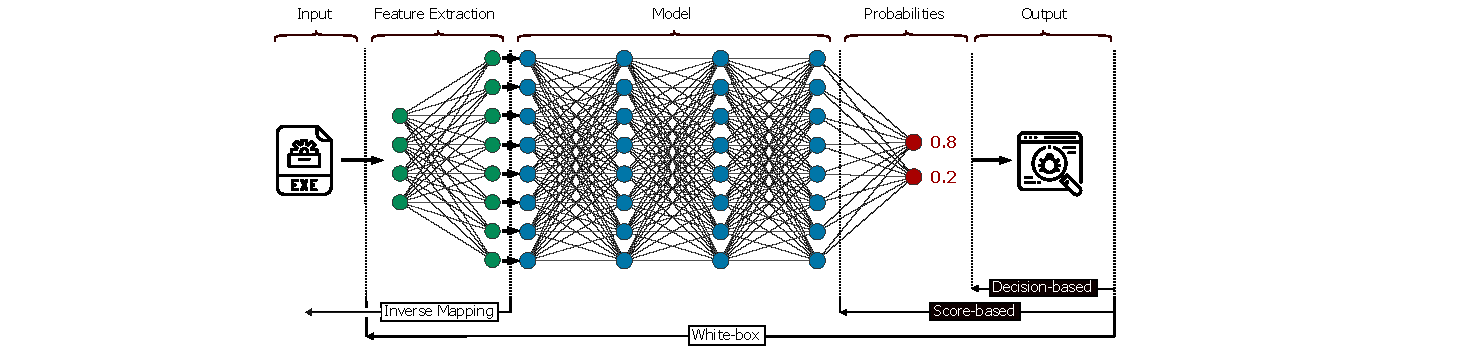
\includegraphics[width=0.99\textwidth]{pipeline.pdf}
    \caption{Abstract neural network based malware detection}
    \label{fig:pipe}
\end{figure}

For these reasons, performing the attacks through the problem space is in some cases preferable, and can lead to a more principled understanding of the vulnerabilities present.
To illustrate the distinction between problem-space and feature-space attacks, as well as situate them in a practical use case, \autoref{fig:pipe} depicts the pipeline of an AI-based malware detection model.
The process starts with a sample in the problem space, which is then transformed into representations in the feature space, which are then processed by the model, to produce probabilities in $[0,1]$ and outputs in the decision space.
The diagram also highlights the varying degrees of access an adversary might have.
Black-box attacks are further divided into score-based and decision-based depending on the adversary's access, to the probabilities or to the discrete decisions respectively.
White-box attacks on the other hand, have a full closed-form description of the model up to the feature representation.
Finally, the inverse mapping is a non-trivial challenge that occurs in all domains where a gap between the problem and the feature space exists.

For real-world deployed models or systems, decision-based attacks remain the most representative and realistic form of adversarial attack.
Our research has therefore focused on black-box and decision-based attacks, aiming to enhance the robustness of models against such threats.
It quickly became apparent that when operating in black-box settings, which cybersecurity environments typically are, the accurate assessment of a system's vulnerability requires adapting and optimizing the attacks used in the evaluation.
Ad-hoc methods or simple heuristics, common in some offensive security research, fail to provide a thorough understanding on the realistic level of threat.
To address this challenge, \gls{RL} represented an ideal framework particularly suited for optimizing objective functions in black-box environments, due to several key characteristics:

\begin{itemize}
    \item Reward Signal Utilization: RL can optimize processes through mere access to scalar feedback from the environment.
    \item Model-Free Nature: Many RL algorithms do not require an explicit model of the environment, making them well-suited for scenarios where such a model is not available or too costly to evaluate.
    \item Exploration-Exploitation Trade-off: RL algorithms inherently balance exploration -- trying new actions to discover their effects -- and exploitation -- using known information to maximize reward.
    \item Sequential Decision-Making: From the adversarial perspective, it is initially uncertain how actions affect the system under attack and its internal states, and the system can respond infrequently or even mislead; thus a methodology than can handle sparse and delayed rewards is advantageous.
    \item Function Approximation: With neural networks parameterizing the policy, RL can handle high-dimensional or continuous state and action spaces.
\end{itemize}


\begin{figure}
    \centering
    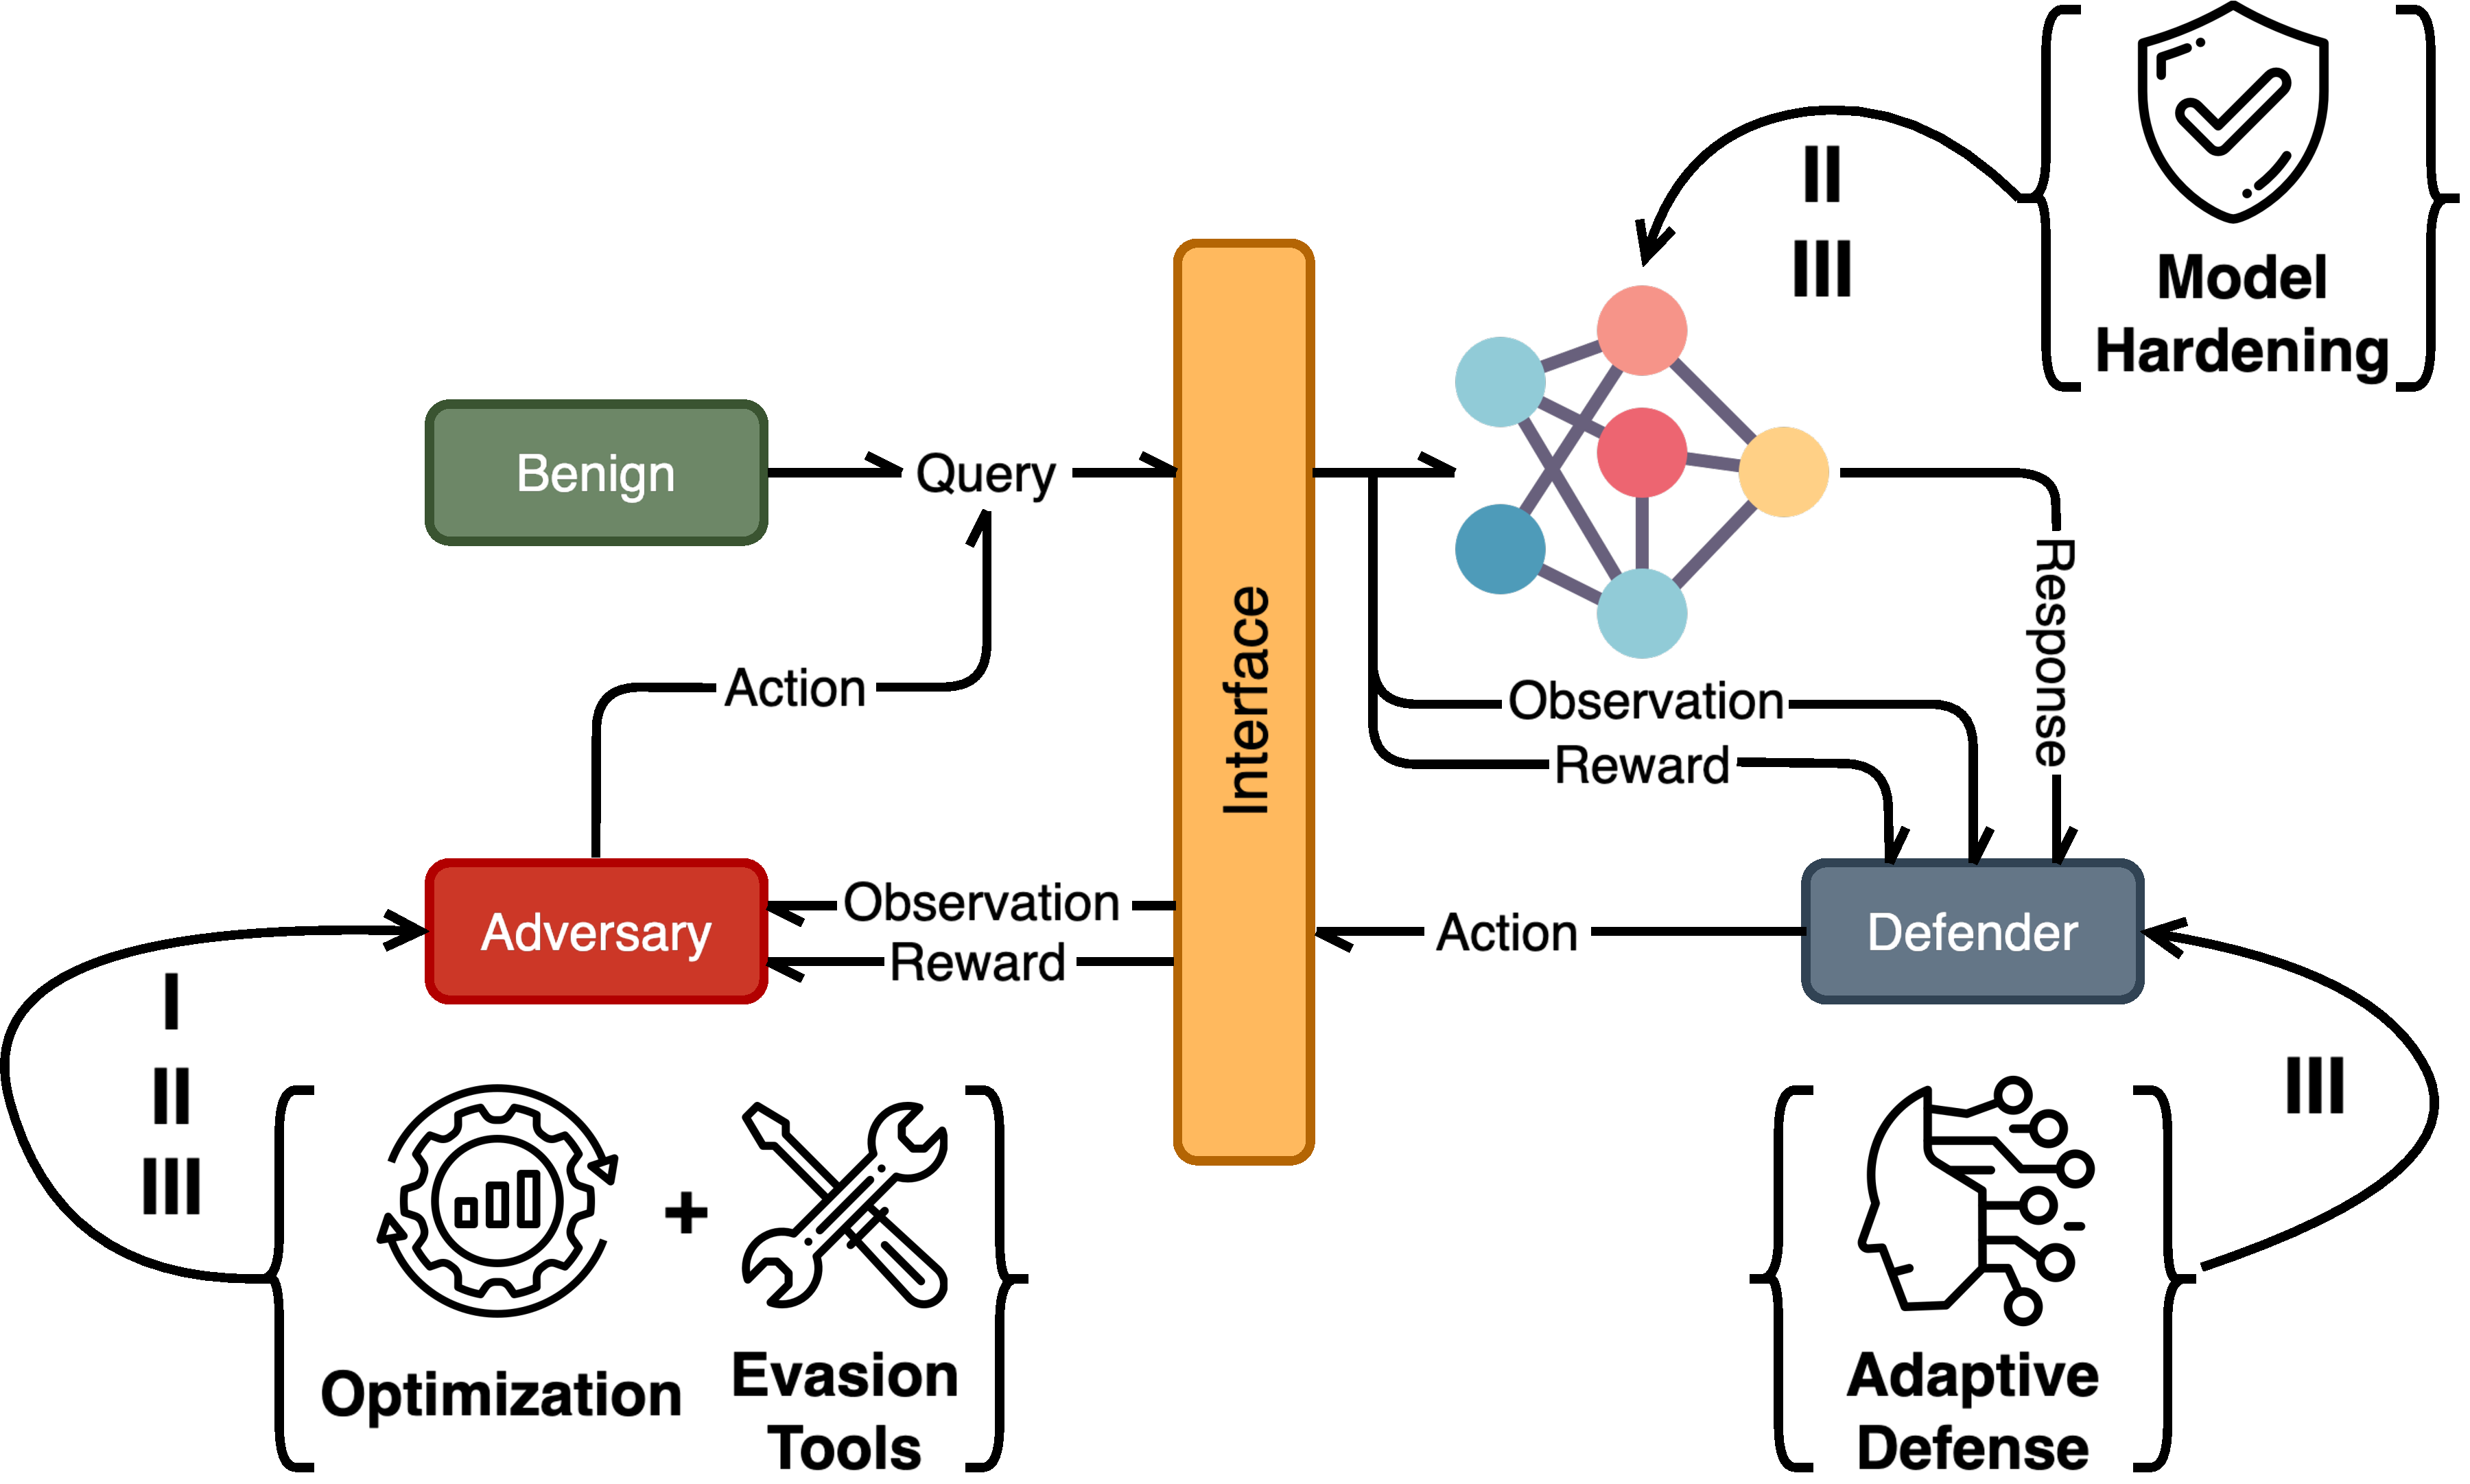
\includegraphics[width=0.99\textwidth]{pillars.pdf}
    \caption[Schematic depiction of an environment that encompasses an AI-based system, black-box attacks, defenses, and all the agents involved.]{Schematic depiction of an environment that encompasses an AI-based system, black-box attacks, defenses, and all the agents involved. We indicate where our three works (I, II, III) are situated with respect to each entity.}
    \label{fig:pillars}
\end{figure}

As outlined earlier, this dissertation centers on three key studies focused on enhancing the security and robustness of AI-based systems against adversarial attacks.
These studies share foundational principles and build progressively upon one another; to situate them within the \gls{AML} landscape, \autoref{fig:pillars} depicts an overview of a conventional environment for black-box attack and defenses, highlighting the specific focus areas of each study.
Our work on Google reCAPTCHA v3, as the investigation of the robustness of a proprietary, real-world system, is in essence the conception, design, and optimization of an adversarial attack against the black-box system, by exploiting the feedback provided by it.
In our second study, with AutoRobust we take problem-space attacks a step further.
As the owners of the detection model now, we use these attacks to adversarially train and strengthen the model against evasion.
Our third study brings these elements together into a unified framework that:
(a) optimizes attacks and their evasion techniques together, (b) hardens models with adversarial training, and (c) adds another defensive layer, namely active and adaptive defenses.
By integrating the above, we evaluate a comprehensive range of scenarios in which both attacks and defenses successively adapt to each other.

In addition to the three core studies, my PhD journey has involved exploring a wide range of research questions in collaboration with colleagues from KU Leuven and international partners.
I had the privilege of conducting a research visit at King's College London and University College London, experiences that were instrumental in shaping my growth both as a researcher and as an individual.
During my PhD, I contributed to several research projects and co-authored a book chapter, all within the realms of \gls{AML} and cybersecurity.
Below, I summarize the research activities relevant to this dissertation that have also led to publications:

\textbf{AutoAttacker: A Reinforcement Learning Approach for Black-box Adversarial Attacks.}
Our initial foray into generating adversarial examples with \gls{RL} was successful, and led to the first publication, a workshop paper accepted at Euro S\&P 2019.
In AutoAttacker, our \gls{RL} agents learn how to evade the black-box model in query-based fashion, by learning a policy for adversarial perturbations.
AutoAttacker was one of the first methodologies to use \gls{RL} for generating adversarial examples in image classification, overcoming challenges associated with non-differentiable models.
This made our approach particularly effective against common defenses at the time, such as gradient obfuscation and masking.  

\begin{myleftbar}
\fullcite{tsingenopoulos2019autoattacker}
\end{myleftbar}

\textbf{Adaptive Malware Control: Decision-Based Attacks in the Problem Space of Dynamic Analysis}
In this study, we redefine adversarial attacks on malware behavior so that they can be performed directly by the original binary and thus obviate the need to compute gradients through feature representations.
We prove theoretically that this can occur even in the fully black-box case where only the final, hard-label decision is disclosed.
Furthermore, we empirically evaluate our approach by training state-of-the-art sequence models for detecting malware behavior, creating several environments for malware manipulation, and training a host of \gls{RL} agents on them that learn evasive policies through interaction.
We then use the adversarial sequences as generated by the RL agents to adversarially train the detection models.
Our results show that while this approach is indispensable, the degree of robustness it imparts can be deceptive; especially when we consider adversaries with broader capabilities.
This work was published the 1st Workshop on Robust Malware Analysis (WoRMA 2022) at AsiaCCS 2022.

\begin{myleftbar}
\fullcite{tsingenopoulos2022adaptive}
\end{myleftbar}

\textbf{Position Paper: On Advancing Adversarial Malware Generation Using Dynamic Features}
At the same workshop, we also presented a position paper on adversarial malware.
We conduct a critical review of existing adversarial attacks against malware detection, and conclude that current research focuses mainly on evasion techniques against static analysis; generating adversarial Windows samples to evade dynamic analysis remains largely unexplored.
In the context of black-box attack scenarios, we investigate an adversary's potential to carry out practical transformations in order to influence the behavioral features observed by ML systems and security products.
Moreover, we investigate the range of dynamic behavior transformations and identify critical properties and associated challenges that relate to feasibility, automation, technical costs and detection risks.
Through this discussion, we propose solutions to important challenges and present promising paths for future research on evasive malware under dynamic analysis.

\begin{myleftbar}
\fullcite{shafiei2022position}
\end{myleftbar}

\textbf{Adversarial Machine Learning}
In collaboration with several colleagues, we co-authored a book chapter on \gls{AI} and security.
While other chapters of the book study the uses of AI in common computer security applications, we focus instead on the field of study concerned with the security of AI algorithms themselves.
\gls{AML} has garnered significant interest from the research community, leading to a wealth of studies that develop either attacks on ML algorithms or defenses against such adversarial strategies.
Notably, adversarial attacks have been explored across nearly all \gls{ML} applications.
Our chapter aims to systematize \gls{AML}, with a practical emphasis on common vulnerabilities.
We introduce the fundamental concepts and core principles of \gls{AML}, without assuming a strong background in \gls{ML}.
This makes the chapter valuable both for security professionals unfamiliar with \gls{ML}, as well as to \gls{ML} researchers seeking to understand the security implications of their work. 

\begin{myleftbar}
\fullcite{hernandez2022adversarial}
\end{myleftbar}

% \textbf{Chained Anomaly Detection Models for Federated Learning: An Intrusion Detection Case Study}
% The major challenge that we address in this work is that in a federated learning setup, an adversary has many more opportunities to poison one of the local machine learning models with malicious training samples, thereby influencing the outcome of the federated learning and evading detection.
% We present a solution where contributing parties in federated learning can be held accountable and have their model updates audited.
% We describe a permissioned blockchain-based federated learning method where incremental updates to an anomaly detection machine learning model are chained together on the distributed ledger.
% By integrating federated learning with blockchain technology, our solution supports the auditing of machine learning models without the necessity to centralize the training data.
% Experiments with a realistic intrusion detection use case and an autoencoder for anomaly detection illustrate that the increased complexity caused by blockchain technology has a limited performance impact on the federated learning, varying between 5 and 15\%, while providing full transparency over the distributed training process of the neural network.
% Furthermore, our federated learning solution can be generalized and applied to more sophisticated neural network architectures and other use cases.

% \begin{myleftbar}
% \fullcite{preuveneers2018chained}
% \end{myleftbar}

% \textbf{Resource Usage and Performance Trade-offs for Machine Learning Models in Smart Environments}
% Finally, we perform a study on multi-objective optimization for ML models, where the best performing model, its architecture and parameters for a given task are ideally automatically determined through a hyperparameter tuning process.
% At the same time, edge computing is an emerging distributed computing paradigm that aims to bring computation and data storage closer to the location where they are needed to save network bandwidth or reduce the latency of requests.
% The challenge we address in this work is that hyperparameter tuning does not take into consideration resource trade-offs when selecting the best model for deployment in smart environments.
% The most accurate model might be prohibitively expensive to computationally evaluate on a resource constrained node at the edge of the network.
% We propose a multi-objective optimization solution to find acceptable trade-offs between model accuracy and resource consumption to enable the deployment of ML models in resource constrained smart environments.
% We demonstrate the feasibility of our approach by means of an anomaly detection use case.
% Additionally, we evaluate the extent that transfer learning techniques can be applied to reduce the amount of training required by reusing previous models, parameters and trade-off points from similar settings.

% \begin{myleftbar}
% \fullcite{preuveneers2020resource}
% \end{myleftbar}

\section{Dissertation Outline}

The remainder of this dissertation is structured as follows:
We begin by providing the necessary background on \gls{AML} and \gls{RL}, where for \gls{RL} we further introduce common algorithms, multi-agent environments, and its relevance for cybersecurity use-cases in Chapter \ref{ch:background}.
In Chapter \ref{ch:recaptcha} we present our first study, the RL-based web automation which successfully bypasses detection by Google reCAPTCHA v3.
Chapter \ref{ch:autorobust} introduces AutoRobust, a methodology of hardening malware detection models against evasion through the problem space.
Chapter \ref{ch:markovgames} explores the intersection of adaptive attacks and defenses, introducing our Adversarial Markov Games (AMG) framework as their composition.
Finally, in Chapter \ref{ch:conclusion} we conclude by summarizing the key contributions and insights of this dissertation, and highlighting open questions and potential directions for future research.

%%%%%%%%%%%%%%%%%%%%%%%%%%%%%%%%%%%%%%%%%%%%%%%%%%
% Keep the following \cleardoublepage at the end of this file, 
% otherwise \includeonly includes empty pages.
\cleardoublepage

% vim: tw=70 nocindent expandtab foldmethod=marker foldmarker={{{}{,}{}}}
